\title{\color{ladrillo}\bfseries Los reyes y los cautiverios\\[4pt]\large\color{cafe}\mdseries Dos reinos, dos destierros y una promesa que vuelve a reunir a todo Israel}
\author{}\date{\color{sepia}Serie «Israel, el pueblo de Dios» · Estudio 5}
\begin{document}
\maketitle\thispagestyle{empty}

\begin{abstract}\noindent
Este quinto estudio recorre la historia del reino dividido, desde la muerte de Salomón hasta la caída de Jerusalén, y muestra que la división desembocó en dos cautiverios distintos: el de Israel, el reino del norte, deportado por Asiria entre 734 y 716 a.\,e.\,c., y el de Judá, el reino del sur, llevado a Babilonia entre 605 y 582 a.\,e.\,c. Las cifras asirias, cotejadas con las estimaciones de población, sugieren que del norte salió en torno a una décima parte de sus habitantes, sobre todo la élite, mientras la mayoría campesina permaneció, se mezcló con colonos o buscó a YHWH en Jerusalén, como atestiguan Crónicas y, con un debate todavía abierto, el crecimiento de la ciudad en los siglos \textsc{viii} y \textsc{vii}. De ahí se sigue que el «todo Israel» de Crónicas, Esdras y Nehemías no designe a doce tribus íntegras ni solo a Judá, sino al pueblo de las doce tribus representado por un remanente. La vocación de «reino de sacerdotes y nación santa» (Éx 19:6) se quiebra en ambos reinos, y en la hora del juicio Isaías, Jeremías, Ezequiel y Oseas anuncian el regreso y la reunión de las dos casas bajo un rey davídico, promesa sobre la que Pablo construirá Romanos~11.
\par\smallskip\noindent\textbf{Palabras clave:} reino dividido, cautiverio asirio, cautiverio babilónico, Samaria, remanente, tribus del norte, todo Israel, nuevo pacto, Ezequiel 37, Romanos 11.
\end{abstract}

\section{Introducción}

¿Qué queda de Israel cuando Israel deja de existir como reino? La pregunta se plantea dos veces en este período, y la respuesta no es la misma. En 722 a.\,e.\,c. cae Samaria y el reino del norte desaparece del mapa político; en 586 a.\,e.\,c. cae Jerusalén y el templo arde. Se suele hablar de «el cautiverio» como si hubiera sido uno solo, pero fueron dos, con imperios, políticas y desenlaces diferentes: el norte no tuvo un regreso organizado y su tierra recibió colonos; Judá fue desterrado como comunidad y volvió con Ciro. Entre ambos destinos quedó una zona intermedia que los textos y la arqueología permiten ver, la de los israelitas del norte que no fueron deportados y que terminaron unidos a Judá.

Los libros de Reyes, escritos para una generación desterrada, leen ambos cautiverios como juicio por la infidelidad al pacto (2~R 17:7--23; 24:3--4). Los profetas añaden lo que la crónica sola no podía decir: el Dios que dispersa es el mismo que reunirá, y reunirá a las dos casas. Siglos después, Pablo recurrirá a los textos de esta etapa para sostener que «no ha desechado Dios a su pueblo, al cual antes conoció» (Ro 11:2).

\begin{nota}[Precisión terminológica: tres sentidos de «Israel»]
Desde la división del reino (1~R 12), «Israel» admite tres usos. \textbf{Israel, reino del norte}, son las diez tribus encabezadas por Efraín, con capitales en Siquem, Tirsa y luego Samaria, que los profetas llaman también «Efraín», «Samaria» o «casa de Israel» (Os 5:3; Am 5:1). \textbf{Judá, reino del sur}, comprende Judá y Benjamín, con Jerusalén y la dinastía de David, a los que se suman levitas y emigrados de otras tribus (2~Cr 11:13--17). \textbf{Israel, el pueblo completo}, son las doce tribus como pueblo del pacto (Jer 31:1; Ez 37:11). Aquí se escribe «Israel (norte)» o «reino del norte» para el primer sentido, «Judá» para el segundo e «Israel (el pueblo)» o «todo Israel» para el tercero, y se indica el sentido cuando un texto lo deja abierto.
\end{nota}


\section{Marco cronológico}

El período va desde la división del reino (c. 931/930 a.\,e.\,c.) hasta el edicto de Ciro (538 a.\,e.\,c.). El reino del norte duró unos dos siglos con nueve dinastías, y de sus diecinueve reyes siete murieron asesinados; Judá duró unos tres siglos y medio con una sola, la de David, sostenida aun bajo reyes infieles «por amor a David mi siervo» (1~R 11:13; 2~R 8:19).

\begin{figure}[!htb]\centering
\begin{tikzpicture}[x=1cm,y=1cm]
\def\X#1{(930-#1)*0.0385}
% eje y marcas
\draw[line width=1.6pt,cafe,-{Latex[length=3mm]}] (-0.2,0) -- (15.6,0);
\foreach \a in {900,850,800,750,700,650,600,550}{\draw[cafe,line width=0.6pt] ({\X{\a}},-0.1) -- ({\X{\a}},0.1);}
\foreach \a in {900,850,750,650,550}{\node[font=\fontsize{5}{6}\selectfont,text=sepia,anchor=north,inner sep=1pt] at ({\X{\a}},-0.1) {\a};}
% profetas: norte arriba, sur abajo
\fill[oro!45] ({\X{870}},0.28) rectangle ({\X{800}},0.48); \node[font=\tiny\itshape,text=cafeosc] at ({\X{835}},0.38) {Elías, Eliseo};
\fill[oro!45] ({\X{765}},0.28) rectangle ({\X{722}},0.48); \node[font=\tiny\itshape,text=cafeosc] at ({\X{743}},0.38) {Amós, Oseas};
\fill[ladrillo!25] ({\X{740}},-0.36) rectangle ({\X{700}},-0.56); \node[font=\tiny\itshape,text=cafeosc] at ({\X{720}},-0.46) {Isaías, Miqueas};
\fill[ladrillo!25] ({\X{627}},-0.36) rectangle ({\X{582}},-0.56); \node[font=\tiny\itshape,text=cafeosc] at ({\X{604}},-0.46) {Jeremías};
\fill[ladrillo!25] ({\X{593}},-0.62) rectangle ({\X{571}},-0.82); \node[font=\tiny\itshape,text=cafeosc,right] at ({\X{571}},-0.72) {Ezequiel};
\node[font=\scriptsize\bfseries,text=cafe,anchor=east] at (15.6,1.2) {Israel (reino del norte)};
\node[font=\scriptsize\bfseries,text=ladrillo,anchor=west] at (-0.2,-2.3) {Judá (reino del sur)};
% eventos norte
\foreach \y/\h/\t in {930/0.9/{División del reino (1~R 12)},885/1.75/{Omri; Samaria capital},841/0.9/{Acab en Qarqar (853); Jehú (841)},790/1.6/{Jeroboam~II (2~R 14:25)},722/0.9/{Galilea (732) y Samaria (722--720) deportadas}}{
  \draw[sepia,line width=0.5pt] ({\X{\y}},0) -- ({\X{\y}},\h);
  \fill[oro] ({\X{\y}},0) circle (3.2pt);
  \node[above,font=\tiny\bfseries,text=cafe,text width=1.6cm,align=center,inner sep=1pt] at ({\X{\y}},\h) {\t};}
% eventos sur
\foreach \y/\h/\an/\t in {872/0.95/north/{Josafat (2~Cr 17)},701/0.95/north/{Ezequías ante Senaquerib},622/0.95/north east/{Reforma de Josías (2~R 22--23)},605/2.0/north east/{Carquemis (605); Joaquín deportado (597)},586/0.95/north west/{Caída de Jerusalén (2~R 25)},538/2.0/north/{Edicto de Ciro (Est. 6)}}{
  \draw[sepia,line width=0.5pt] ({\X{\y}},0) -- ({\X{\y}},-\h);
  \fill[ladrillo] ({\X{\y}},0) circle (3.2pt);
  \node[anchor=\an,font=\tiny\bfseries,text=ladrillo,text width=1.45cm,align=center,inner sep=1pt] at ({\X{\y}},-\h) {\t};}
\end{tikzpicture}\\[2pt]
{\footnotesize\color{sepia}\textit{Nota.} Elaboración propia. Fechas aproximadas según Thiele (1983); arriba, el reino del norte; abajo, Judá; las bandas indican la actividad de los profetas.}
\end{figure}

Algunas fechas siguen en discusión sin alterar la secuencia: muchos proponen la toma de Samaria en 722 y la deportación principal en 720 (Becking, 1992), y la caída de Jerusalén se fecha en 586 (Thiele) o en 587 a.\,e.\,c.

\section{Contexto histórico y arqueológico}

\subsection{Dos imperios, dos políticas}
En el siglo \textsc{ix} a.\,e.\,c. Israel (norte) fue una potencia regional, rival de Aram-Damasco. Desde Tiglat-pileser~III (745--727), Asiria dejó de conformarse con el tributo: anexaba los reinos rebeldes como provincias y deportaba poblaciones en ambas direcciones, trasladando a los vencidos a otras regiones del imperio y trayendo a su tierra gente de otros países, con el fin de quebrar las identidades nacionales (Younger, 1998). El reino del norte cayó bajo ese sistema. Babilonia, que heredó el imperio tras Carquemis (605), deportó a las élites de Judá y las asentó en comunidades propias, pero no trajo colonos extranjeros a Judá. Esa diferencia de política explica en buena parte por qué los desterrados de Judá conservaron su identidad y pudieron regresar como pueblo, mientras los del norte se dispersaron.

\subsection{El reino del norte en las inscripciones}
Las fuentes extrabíblicas iluminan sobre todo los siglos de poder del norte. La Estela de Mesa (c. 840 a.\,e.\,c.) recuerda que «Omri era rey de Israel y oprimió a Moab muchos días» (cf. 2~R 3:4--5), y el Obelisco Negro muestra a «Jehú, hijo de Omri» postrado ante Salmanasar~III en 841. Los ostracones de Samaria, de la primera mitad del siglo \textsc{viii}, muestran nombres con \emph{-yau} (YHWH) junto a nombres formados con Baal, el sincretismo que denuncia Oseas (Os 2:16--17 [2:18--19]).



El final del reino tiene también su documentación asiria. Tiglat-pileser~III registra el tributo de «Menahem de Samaria» (2~R 15:19) y afirma que, derrocado Peka, puso a Oseas como rey (cf. 2~R 15:30). Sus anales cuentan además 13.520 cautivos tras «arrasar 16 distritos» de Israel, sobre todo en la Baja Galilea, y un fragmento enumera cautivos de ciudades galileas como Hanatón, Jotba, Ruma y Merom (Younger, 2003). Los anales de Sargón~II dicen: «sitié y conquisté Samaria; llevé cautivos a 27.290 habitantes» (el Prisma de Nimrud da 27.280), y añaden que repobló la provincia de «Samerina» con gente de otros países conquistados (Pritchard, 1969; cf. 2~R 17:24).

\subsection{Judá en las inscripciones}
De Judá la arqueología conserva sobre todo la crisis. El Prisma de Senaquerib dice que tomó 46 ciudades de «Ezequías el judaíta» y lo encerró «como a un pájaro en su jaula, en Jerusalén», pero no afirma haber tomado la ciudad (cf. 2~R 19:32--36); los relieves de Laquis narran el asedio de 701, cuya rampa asiria se excavó en el sitio (Ussishkin, 1982). Del destierro hablan dos hallazgos que importan para la restauración: unas tablillas de raciones del palacio de Babilonia nombran a «Ya'ukinu, rey de Yahudu», Joaquín, cuya liberación cierra el libro de Reyes con una luz de esperanza (Weidner, 1939; 2~R 25:27--30), y las tablillas de Al-Yahudu, «ciudad de Judá», contratos de una aldea babilónica entre c. 572 y 477, muestran nombres yahvistas durante generaciones y dan cuerpo al consejo de Jer 29:5--7 (Pearce y Wunsch, 2014).

\begin{center}\begin{minipage}{\linewidth}\centering
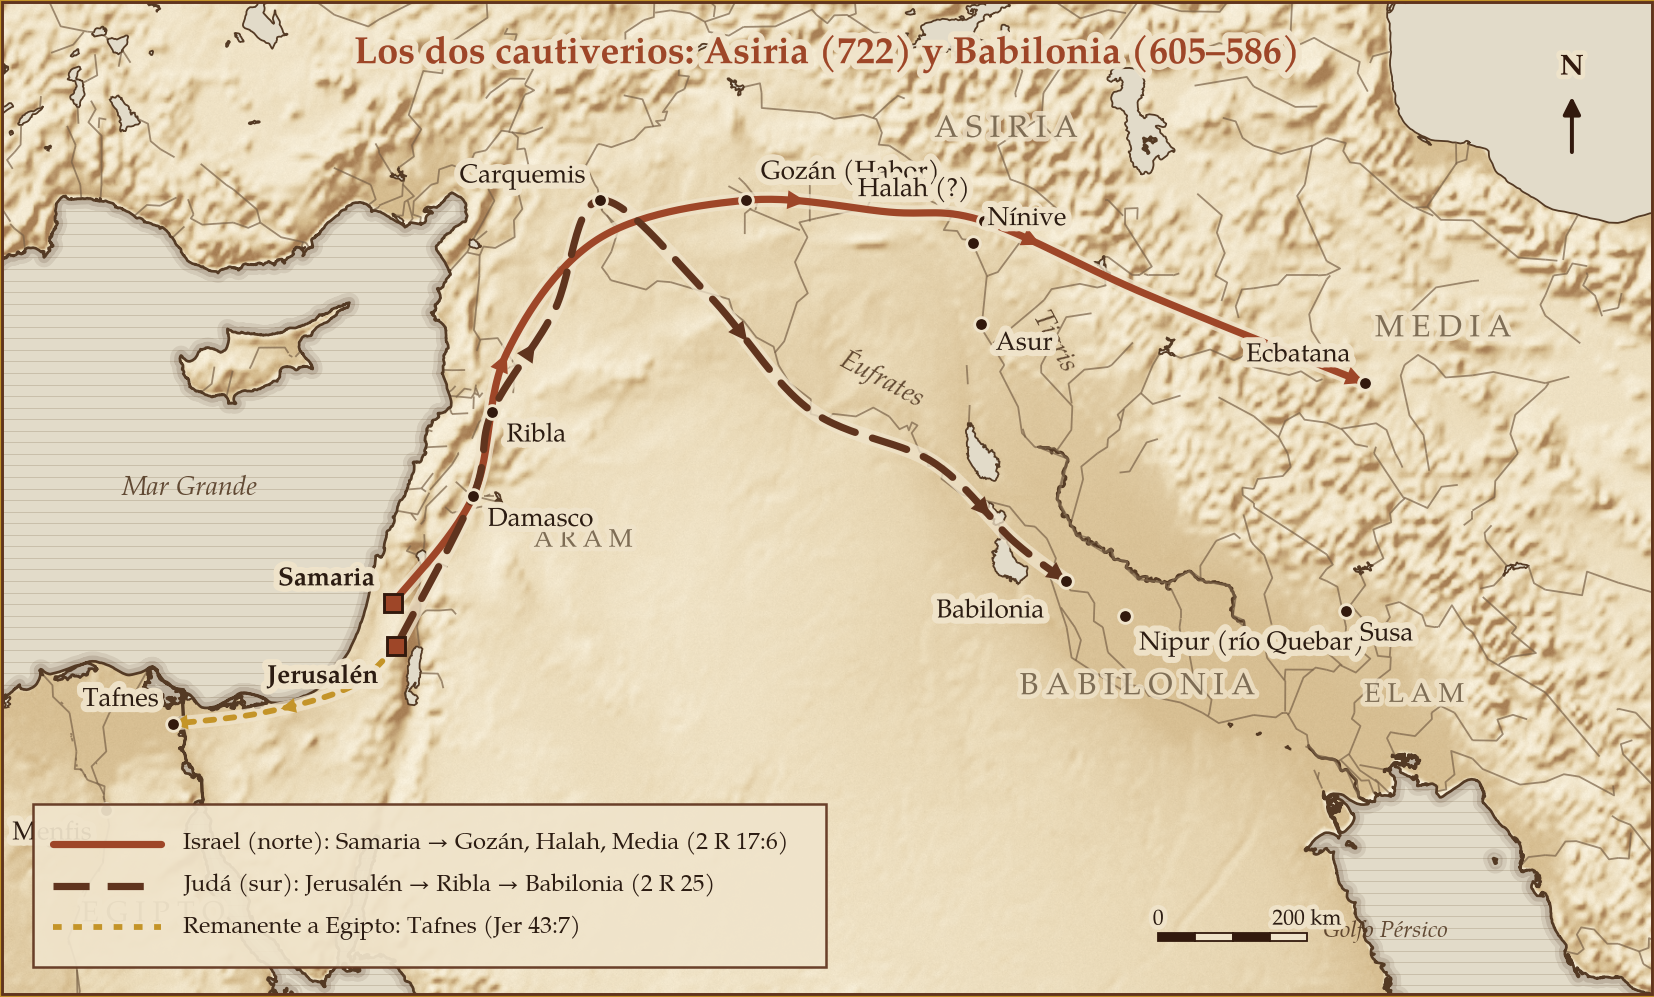
\includegraphics[width=0.82\linewidth]{mapa_cautiverios.png}\\[2pt]
{\footnotesize\color{sepia}\textit{Nota.} Elaboración propia: costas, lagos y ríos GSHHS/WDB y relieve sombreado (Basemap); ubicaciones antiguas aproximadas. La ubicación de Halah es incierta.}
\end{minipage}\end{center}

\section{Desarrollo bíblico}

\subsection{El reino del norte: un trono sin pacto}
Dios ofrece a Jeroboam una «casa firme, como la que edifiqué a David», si guarda sus mandamientos (1~R 11:38). Jeroboam, temiendo que el templo de Jerusalén devuelva el pueblo a la casa de David, levanta becerros de oro en Betel y en Dan (1~R 12:28--33), y «el pecado de Jeroboam, que hizo pecar a Israel» será el estribillo con que Reyes juzga a todos los reyes del norte.

La respuesta fue una primera migración hacia el sur. Sacerdotes, levitas y, «de todas las tribus de Israel, los que habían dispuesto su corazón a buscar a YHWH», vinieron a Jerusalén (2~Cr 11:13--16), y bajo Asa llegaron más de Efraín, Manasés y Simeón (2~Cr 15:9). Desde el principio, Judá fue el lugar donde se reunían los fieles de todas las tribus, un dato que reaparecerá al hablar del «todo Israel» posexílico.

\subsection{Elías y el remanente de los siete mil}
En el Carmelo, Elías plantea al reino del norte una elección: «¿Hasta cuándo saltaréis entre dos ramas? Si YHWH es Dios, seguidle; y si Baal, seguidle a él» (1~R 18:21). Reconstruye el altar «con doce piedras, conforme al número de las tribus de los hijos de Jacob» (18:31), afirmando en pleno reino del norte que Israel sigue siendo un pueblo de doce tribus. Después, amenazado por Jezabel, huye al Horeb convencido de que «solo yo he quedado» (19:10), y la respuesta divina corrige su percepción:
\begin{cita}Y haré que queden en Israel siete mil: todas las rodillas que no se doblaron ante Baal y todas las bocas que no lo besaron.\fuente{(1~R 19:18)}\end{cita}
El remanente existe porque Dios lo deja, y Pablo lee aquí la clave de su propio tiempo: «así también, en el tiempo presente, ha quedado un remanente escogido por gracia» (Ro 11:5).

\subsection{Amós y Oseas: profetas para el norte}
Bajo Jeroboam~II (793--753) el norte alcanzó su mayor extensión desde Salomón, y el narrador atribuye esa prosperidad a la misericordia: «YHWH no había dicho que borraría el nombre de Israel de debajo del cielo» (2~R 14:27). Sobre esa prosperidad levantada en la injusticia predica \textbf{Amós} en Betel, y anuncia que Dios zarandeará a la casa de Israel entre las naciones «como en una criba, y no caerá un grano a tierra» (Am 9:9).

\textbf{Oseas}, el único profeta escritor del norte, convierte su matrimonio con Gómer en parábola. Su tercer hijo se llama \emph{Lo-Ammí}, «no mi pueblo» (Os 1:9), nombre que invierte la fórmula del pacto (Lv 26:12); pero la sentencia se revierte apenas pronunciada, y en el lugar donde se les dijo «No sois mi pueblo» se les dirá «Hijos del Dios viviente» (1:10 [2:1]). Oseas distingue con cuidado: Dios no se compadecerá más de la casa de Israel (norte), pero sí de la de Judá (1:6--7), y luego promete que las dos casas se reunirán bajo «una sola cabeza» (1:11 [2:2]). Pablo cita estos versículos en Ro 9:25--26 y los aplica también a los gentiles llamados (9:24), por analogía: si Dios pudo llamar «mi pueblo» a quienes había declarado «no mi pueblo», puede llamar también a quienes nunca lo fueron (Moo, 1996; Hays, 1989).

\subsection{Dos cautiverios distintos}\label{sec:doscautiverios}

\subsubsection*{El cautiverio asirio del reino del norte}
El cautiverio del norte no fue un acontecimiento, sino un proceso de casi dos décadas. Comenzó en 733--732, cuando Tiglat-pileser~III respondió a la alianza de Peka de Israel con Aram contra Asiria: tomó las ciudades de Neftalí y «llevó a todos cautivos a Asiria» (2~R 15:29), y deportó también a rubenitas, gaditas y a la media tribu de Manasés de Transjordania (1~Cr 5:6, 26), que Malamat (2007) identifica con «los jefes de clanes». El reino quedó reducido a las colinas de Efraín y Manasés en torno a Samaria. Oseas hijo de Ela, puesto como vasallo, buscó luego la ayuda de Egipto y dejó de pagar tributo, y Salmanasar~V sitió Samaria tres años:
\begin{cita}En el año noveno de Oseas, el rey de Asiria tomó Samaria y llevó a Israel cautivo a Asiria, y los puso en Halah, en el Habor, río de Gozán, y en las ciudades de los medos.\fuente{(2~R 17:6; cf. 18:10--11)}\end{cita}
La deportación principal la hizo Sargón~II en 720, y la repoblación continuó durante décadas: en 716/715 Sargón asentó tribus árabes en la tierra de «Bit-Humri», la «casa de Omri» (Malamat, 2007; Younger, 2003), y Esd 4:2 y 4:9--10 recuerdan colonos traídos más tarde por Asarhadón y por «Asenapar», probablemente Asurbanipal.

\begin{perla}{el sermón de 2 R 17}
El narrador detiene el relato de la caída de Samaria para explicarla, y su vocabulario convierte el destierro en un Éxodo deshecho que mira también a Judá.\par\smallskip
{\centering\renewcommand{\arraystretch}{1.15}
\begin{tabular}{>{\RaggedRight\arraybackslash}p{1.6cm}>{\RaggedRight\arraybackslash}p{5.9cm}>{\RaggedRight\arraybackslash}p{6.4cm}}
\toprule
\textbf{Texto} & \textbf{Formulación} & \textbf{Observación}\\
\midrule
17:7 & Pecaron contra YHWH, «que los sacó de la tierra de Egipto» & El destierro invierte el Éxodo\\
17:13 & \heb{שֻׁבוּ מִדַּרְכֵיכֶם הָרָעִים} «Volveos de vuestros malos caminos», dicho «a Israel y a Judá» & En el centro del juicio está el verbo del regreso, \emph{shuv}\\
17:15 & \heb{וַיֵּלְכוּ אַחֲרֵי הַהֶבֶל וַיֶּהְבָּלוּ} «siguieron la vanidad y se hicieron vanos» & Juego \emph{hével}/\emph{yehbalú}: se vuelve uno lo que adora (Jer 2:5)\\
17:18--20 & «No quedó sino la tribu de Judá», pero «tampoco Judá guardó los mandamientos» & «Israel» pasa del reino del norte al pueblo completo: el sermón anuncia ya el destierro de Judá\\
17:23 & \heb{וַיִּגֶל יִשְׂרָאֵל מֵעַל אַדְמָתוֹ} «fue llevado Israel cautivo de su tierra» & \emph{galá}, el verbo del exilio\\
\bottomrule
\end{tabular}\par}
\smallskip
Escrito para desterrados de Judá, el sermón no cierra la historia: la misma llamada a «volver» que el pueblo desoyó es la que los profetas convertirán en promesa de regreso.
\end{perla}

\subsubsection*{El cautiverio babilónico de Judá}
El de Judá fue también escalonado, pero siguió otra lógica. En 605, tras vencer a Egipto en Carquemis (Jer 46:2), Nabucodonosor llevó a Babilonia a jóvenes nobles, entre ellos Daniel (Dn 1:1--6). En 597 se rindió Joaquín y fue deportado con la corte, los guerreros y los artesanos, unos diez mil (2~R 24:12--16), entre ellos el sacerdote Ezequiel (Ez 1:2--3). Sedequías se rebeló, y en 586 Jerusalén cayó tras un largo asedio; Nebuzaradán quemó el templo y la ciudad y deportó al resto, «dejando a los pobres como viñadores» (2~R 25:8--12; Jer 52:12--16). Tras el asesinato de Gedalías, un resto huyó a Egipto (Jer 40--44), y Jer 52:30 registra una última deportación en 582. Babilonia no trajo colonos: la tierra quedó empobrecida pero no repoblada, y los desterrados vivieron agrupados junto al río Quebar o en aldeas como Al-Yahudu.

\begin{table}[!htbp]\centering\footnotesize
\renewcommand{\arraystretch}{1.12}
\begin{tabular}{>{\RaggedRight\arraybackslash}p{2.3cm}>{\RaggedRight\arraybackslash}p{6.0cm}>{\RaggedRight\arraybackslash}p{6.0cm}}
\toprule
& \textbf{Israel (norte) bajo Asiria} & \textbf{Judá bajo Babilonia}\\
\midrule
Fechas & 733--732 (Galilea, Galaad); 722--720 (Samaria); colonos en 716/715 y hasta c. 670 & 605 (nobles, Daniel); 597 (Joaquín, Ezequiel); 586 (Sedequías, templo); 582\\
Imperio & Neoasirio: Tiglat-pileser~III, Salmanasar~V, Sargón~II & Neobabilónico: Nabucodonosor~II\\
Textos & 2~R 15:29; 17:1--41; 18:9--12; 1~Cr 5:6, 26; Os; Am & 2~R 24--25; 2~Cr 36; Jer 39--44; 52; Dn 1; Ez 1--24; Lm\\
Deportados & 13.520 (Tiglat-pileser~III) y 27.290 (Sargón~II): unos 41.000 documentados, quizá un 10--15 \% de la población & c. 10.000 en 597 (2~R 24:14--16); Jer 52:28--30: 3.023, 832 y 745 (quizá solo varones adultos)\\
Quiénes & Élite, corte, soldados, escribas, artesanos; Galilea casi vaciada; campesinado de las colinas en su tierra & Rey, corte, sacerdotes, guerreros, artesanos; «los pobres de la tierra» quedan (2~R 25:12)\\
Repoblamiento & Colonos de Babilonia, Cuta, Hamat y otros (2~R 17:24); tribus árabes & Ninguno; tierra empobrecida, no repoblada\\
Destino & Habor, Gozán, Media; asimilación de muchos; en la tierra, mezcla con colonos y origen de los samaritanos; parte se une a Judá & Comunidades agrupadas (Quebar, Al-Yahudu); identidad conservada; en Egipto, Tafnes y después Elefantina\\
Regreso & Ningún regreso organizado; individuos y familias integrados a Judá; promesa pendiente (Is 11:11--13; Ez 37:15--22) & Edicto de Ciro, 538 (Esd 1); Zorobabel, Esdras, Nehemías (Estudio~6)\\
\bottomrule
\end{tabular}\end{table}

\subsection{¿Cuántos fueron deportados del norte, y quiénes?}
Las cifras asirias permiten un cálculo aproximado, que conviene presentar como estimación y no como dato. Los anales suman unos 41.000 deportados: 13.520 de Tiglat-pileser~III y 27.290 de Sargón~II, en deportaciones escalonadas entre c. 734 y 716 (Younger, 2003). Broshi y Finkelstein (1992) calculan para fines del siglo \textsc{viii} unos 400.000 habitantes al oeste del Jordán, de los cuales unos 110.000 vivían en las colinas de Judá, Benjamín y Jerusalén; para el reino del norte cabe hablar, con prudencia, de unos 350.000. Sobre esa base, la deportación documentada equivale a algo así como un 10 a 15 \% de la población del norte. La cifra tiene dos límites: las inscripciones reales son propaganda y pueden estar redondeadas o infladas, y Salmanasar~V pudo deportar a otros sin dejar registro (Younger, 2003).

El promedio oculta, además, una distribución muy desigual. Zvi Gal estimó la población de la Baja Galilea antes de la invasión en unos 17.600 habitantes (Gal, 1992); con los muertos de la campaña y 13.520 deportados, Younger (2003) concluye que la región quedó «prácticamente arrasada», y la arqueología confirma allí un fuerte descenso de población después de 732. Las colinas de Samaria, de Efraín y de Manasés, en cambio, muestran más continuidad en sus aldeas (Becking, 1992) y conservaron la mayor parte de su población rural.

Tampoco se deportaba a cualquiera. La práctica asiria se llevaba sobre todo a la aristocracia, a la corte, a los escribas, a los soldados y a los artesanos, con sus familias, y dejaba al campesinado para que siguiera trabajando la tierra y pagando tributo (Malamat, 2007). Sargón~II incorporó a su ejército un cuerpo de carros «samaritano» (Dalley, 1985). Lo que desapareció en 722, por tanto, fue sobre todo el Estado del norte: su rey, su administración, su ejército y su clase dirigente. La mayoría del pueblo siguió en la tierra.

\subsection{Los deportados en Asiria}
Los textos sitúan a los deportados en la Alta Mesopotamia, junto al Habor, cerca de Gozán (Tell Halaf), y desde 716 algunos en las ciudades de Media (2~R 17:6; 18:11; Malamat, 2007). Los documentos de Gozán conservan nombres yahvistas, terminados en \emph{-yau}, como los de los funcionarios Palti-yau y Neri-yau, y una lista de vino asigna raciones a sacerdotes samaritanos (Younger, 2003), aunque muchos nombres semíticos del noroeste podrían ser arameos o fenicios (Malamat, 2007). Los deportados no eran esclavos, y muchas familias se asirianizaron en pocas generaciones (Younger, 2003); otras conservaron su identidad y terminaron fundiéndose con el exilio judaíta (Malamat, 2007). Josefo dirá en el siglo \textsc{i} que las diez tribus seguían «más allá del Éufrates, una multitud inmensa» (\emph{Ant.} 11.5.2 [11.133]).

\subsection{Los que quedaron en el norte}
De los que no fueron deportados se ocupan dos tradiciones que no se excluyen. Reyes cuenta que Asiria trajo gente de Babilonia, Cuta, Ava, Hamat y Sefarvaim y la estableció «en las ciudades de Samaria en lugar de los hijos de Israel» (2~R 17:24); un sacerdote israelita desterrado volvió a Betel para enseñarles, y el resultado fue un culto mixto: «temían a YHWH y servían a sus dioses» (17:33). Los samaritanos, por su parte, se llaman \emph{shamerim}, «guardianes» de la Torá, y se consideran descendientes de Efraín y Manasés que nunca dejaron la tierra. Las dos versiones tienen fundamento: hubo colonos, pero buena parte de la población rural israelita permaneció, se mezcló con ellos y mantuvo el culto a YHWH. En 407 a.\,e.\,c. la comunidad judía de Elefantina escribió a Delaías y Selemías, hijos de Sanbalat, gobernador de Samaria, y los nombres yahvistas de esa familia muestran la continuidad del yahvismo en la élite samaritana del período persa (papiro de Elefantina; Cowley, 1923, n.º 30).

Crónicas, en cambio, mira a los israelitas del norte que siguieron buscando a YHWH en Jerusalén. Ezequías envió cartas a Efraín y Manasés para invitarlos a la Pascua: «volveos a YHWH [\ldots] y él se volverá al remanente que ha quedado de la mano de los reyes de Asiria» (2~Cr 30:6). Muchos se burlaron de los mensajeros, pero vinieron hombres de Aser, Manasés, Zabulón e Isacar (30:10--11, 18). Josías llevó su reforma hasta Betel y «las ciudades de Samaria» (2~R 23:15--20), purificó las ciudades de Manasés, Efraín y Simeón hasta Neftalí (2~Cr 34:6) y recibió para el templo ofrendas «de Manasés, de Efraín y de todo el remanente de Israel» (34:9); su Pascua reunió, dice el cronista, a todo Judá y a los de Israel que se encontraban allí (35:18). Aun después de 586, ochenta hombres de Siquem, Silo y Samaria subieron con ofrendas a la casa de YHWH (Jer 41:5). Para estos israelitas el centro del culto era Jerusalén, y la Pascua y el templo fueron el camino por el que el remanente del norte volvió a unirse a Judá.

\subsection{Del norte a Judá: lo que dicen los textos y lo que discuten los arqueólogos}
La Biblia atestigua así una corriente continua de israelitas del norte hacia Judá, antes de 722 (2~Cr 11:13--17; 15:9), después (2~Cr 30; 34--35) y tras el exilio, cuando en Jerusalén habitaron «hijos de Judá, de Benjamín, de Efraín y de Manasés» (1~Cr 9:3). Ni Reyes ni Crónicas, sin embargo, narran una huida masiva en 722: Crónicas habla de invitaciones, peregrinaciones y grupos que «se humillaron y vinieron a Jerusalén» (2~Cr 30:11).

La arqueología añade un dato llamativo. En los siglos \textsc{viii} y \textsc{vii} Jerusalén pasó de unas 10 o 12 hectáreas a unas 60, al ocupar la colina occidental, protegida por el muro ancho que se ha relacionado con Is 22:10, y el barrio nuevo que 2~R 22:14 llama «Mishné»; Broshi (1974) estimó que la ciudad triplicó o cuadruplicó su tamaño, y las cifras de habitantes que circulan, de unos 5.000 a unos 25.000, son estimaciones a partir de la superficie habitada. Finkelstein (2008, 2015) atribuye buena parte de ese crecimiento a israelitas del norte llegados después de 720, y con ello explica cómo entraron en la Biblia hebrea tradiciones del norte, como Oseas, Amós, los relatos de Jacob y de Betel. Na'aman (2007, 2014) lo niega: la colina occidental ya estaba ocupada antes, en Judá faltan nombres en \emph{-yau} típicos del norte, los artefactos de estilo israelita son escasos, y muchos de los recién llegados serían más bien judaítas de la Sefelá desplazados por la campaña de Senaquerib en 701. Schniedewind (2004) propone una posición intermedia: quienes vinieron del norte fueron sobre todo escribas, sacerdotes y funcionarios, pocos en número pero decisivos para la transmisión de sus tradiciones.

Lo honesto es reconocer ambos lados. Que hubo migración del norte a Judá lo afirman los textos, y la arqueología lo hace verosímil; su magnitud, en cambio, sigue en discusión, y no conviene apoyar la teología en una cifra que los especialistas no comparten.

\subsection{«Todo Israel» en Crónicas, Esdras y Nehemías}
Con estos datos se puede responder a una pregunta que el lector de los libros posexílicos se hace con razón. Cuando Neh 12:47 dice que «todo Israel», en días de Zorobabel y en días de Nehemías, entregaba las porciones de los cantores y porteros, o cuando Esd 8:35 cuenta que los que volvieron con Esdras ofrecieron doce becerros «por todo Israel», ¿se trata de las doce tribus o de un pequeño resto de Judá?

Los textos no dicen ni lo uno ni lo otro. Crónicas usa «todo Israel» para el pueblo de las doce tribus como unidad, y presenta a Judá como el núcleo al que se incorporan los fieles de todas ellas (Williamson, 1977). Esdras y Nehemías siguen ese modo de pensar: en la dedicación del templo se ofrecen doce machos cabríos «conforme al número de las tribus de Israel» (Esd 6:17), y la ofrenda de Esd 8:35 se hace en nombre de todo el pueblo. La comunidad que volvió era mayoritariamente de Judá, Benjamín y Leví, como reconoce Neh 11:3--4 al nombrar a «Israel, sacerdotes, levitas» y a los hijos de Judá y de Benjamín, pero incluía descendientes del norte asimilados a ella (1~Cr 9:3), y se entendía a sí misma como representante de las doce tribus. El «todo Israel» posexílico no es, pues, un censo de doce tribus íntegras que habrían vuelto, ni tampoco un nombre que se apropia Judá solo: es el pueblo de las doce tribus presente en un remanente que reúne a miembros de varias de ellas. El Nuevo Testamento conserva esa conciencia, con Ana «de la tribu de Aser» (Lc 2:36) y la esperanza de «nuestras doce tribus» (\grc{τὸ δωδεκάφυλον ἡμῶν}, Hch 26:7; cf. Stg 1:1).

Esta lectura descarta también dos simplificaciones sobre las «tribus perdidas». Las diez tribus no desaparecieron sin dejar rastro, porque buena parte del norte quedó en la tierra o se unió a Judá; tampoco se conservaron intactas en algún rincón del mundo, porque muchos deportados se asimilaron. La llamada teoría de las Dos Casas, que identifica a muchos gentiles creyentes con descendientes de Efraín, tiene el mérito de tomar en serio que los profetas prometen reunir a dos casas, pero carece de apoyo: «Judá» ya incluía a israelitas de todas las tribus, la «multitud de naciones» de Gn 48:19 no es el «pleroma de los gentiles» de Ro 11:25, y Pablo funda la inclusión de los gentiles en el llamado y la fe (Ro 9:24, 30), no en una genealogía oculta. El sentido colectivo y representativo del «todo Israel» posexílico prepara, en cambio, el de \grc{πᾶς Ἰσραήλ} en Ro 11:26, que se examinará en el Estudio~8.

\section{Israel como nación santa y reino de sacerdotes}

Éx 19:5--6 había ligado el llamado de Israel a la obediencia, y los profetas describen cómo se quiebra esa vocación en los dos reinos: el culto se separa de la justicia (Is 1:11--15; Am 2:6), el templo se trata como amuleto (Jer 7:4) y Oseas lo dice en términos sacerdotales: «Por cuanto tú desechaste el conocimiento, yo te desecharé para que no seas mi sacerdote» (Os 4:6).

La vocación, sin embargo, no se extinguió. La preservaron los siete mil de Elías, los fieles del norte que buscaron a YHWH en Jerusalén (2~Cr 11:16; 30:11) y el pequeño remanente de Is 1:9, que Pablo cita en Ro 9:29. La preservaron los desterrados de Judá, a quienes Jeremías pidió: «Procurad la paz de la ciudad adonde os hice transportar, y rogad por ella a YHWH» (Jer 29:7). Daniel, al leer a Jeremías, confiesa los pecados de «todo Israel, los de cerca y los de lejos» (Dn 9:7), una oración que abarca a las dos casas.

\section{Aporte de la tradición judía}

La memoria judía de esta etapa vive sobre todo en el calendario de ayunos y en la reflexión rabínica sobre las causas de la destrucción y sobre el destino del norte; lo que sigue pertenece a la tradición y no al texto bíblico. El 9 de Av (\emph{Tishá be-Av}) es el duelo por los dos templos. Ese día se lee Lamentaciones, \emph{Eijá}, y al final se repite 5:21 para no concluir con el lamento de 5:22:
\begin{cita}Haznos volver, YHWH, a ti, y volveremos; renueva nuestros días como al principio.\fuente{(Lm 5:21)}\end{cita}
El verbo \emph{shuv} aparece dos veces y en ese orden: primero Dios hace volver, después el pueblo vuelve. Tras Tisha be-Av se leen siete haftarot de consolación de Is 40--66, comenzando por «Consolad, consolad a mi pueblo» (Is 40:1), y así el año litúrgico conduce del lamento a la promesa.

Sobre las diez tribus, la tradición no ofrece una respuesta única. La Mishná conserva un debate:
\begin{cita}Las diez tribus no han de volver, pues está dicho: «y los arrojó a otra tierra, como en este día» (Dt 29:28 [29:27]). Así como el día se va y no vuelve, también ellas se fueron y no vuelven. Palabras de Rabí Akiva. Rabí Eliézer dice: así como el día oscurece y vuelve a aclarar, así a las diez tribus, para las que oscureció, les volverá a aclarar.\fuente{(Mishná, Sanedrín 10:3)}\end{cita}
Rabí Akiva se apoya en el carácter definitivo del juicio de Dt 29; Rabí Eliézer, en los profetas que anuncian la reunión de las dos casas (cf. Talmud, Sanedrín 110b). La oración diaria se inclina por la esperanza: la décima bendición de la Amidá pide «reúnenos juntos de los cuatro extremos de la tierra. Bendito eres tú, YHWH, que reúnes a los dispersos (\heb{נִדְחֵי}) de tu pueblo Israel» (Sacks, 2009), con el lenguaje de Is 11:12, y el Targum de Isaías liga esa restauración al Mesías davídico al leer Is 11:1 en clave mesiánica (Chilton, 1987).

\section{La promesa de restauración}

Ninguna etapa de la historia de Israel formula la promesa con tanto detalle como la del juicio, y ninguna la dirige con tanta precisión a las dos casas.

\subsection{Isaías: el remanente volverá y Efraín se reconciliará con Judá}
El hijo de Isaías se llamaba \emph{Shear-yashuv}, «un remanente volverá» (Is 7:3), y en 10:21 el nombre se vuelve profecía:
\begin{cita}Un remanente volverá, el remanente de Jacob, al Dios fuerte. Porque aunque tu pueblo, Israel, fuere como la arena del mar, solo un remanente de él volverá.\fuente{(Is 10:21--22)}\end{cita}
\heb{אֵל גִּבּוֹר} («Dios fuerte») es el título del niño davídico de Is 9:6 [9:5], y Pablo cita el texto en Ro 9:27--28. La palabra encierra juicio, porque solo vuelve un remanente, y esperanza, porque ese remanente ciertamente vuelve. Un capítulo después, Isaías habla con más claridad que nadie de la reunión de las dos casas:
\hebverso{וְאָסַף נִדְחֵי יִשְׂרָאֵל וּנְפֻצוֹת יְהוּדָה יְקַבֵּץ מֵאַרְבַּע כַּנְפוֹת הָאָרֶץ}
\begin{cita}Alzará pendón a las naciones, y reunirá a los desterrados de Israel, y juntará a los esparcidos de Judá de los cuatro confines de la tierra. Y se disipará la envidia de Efraín [\ldots]; Efraín no tendrá envidia de Judá, ni Judá afligirá a Efraín.\fuente{(Is 11:12--13)}\end{cita}
El paralelismo distingue a los «desterrados» (\emph{nidjé}) de Israel, el norte deportado por Asiria, y a los «esparcidos» (\emph{nefutsot}) de Judá. La reunión es «por segunda vez» (11:11), desde Asiria, Egipto y las costas, y la encabeza el «renuevo del tronco de Isaí» (11:1, 10). Más adelante el Siervo recibirá la misión de «levantar las tribus de Jacob», no únicamente a Judá, y ser «luz de las naciones» (49:6).

\subsection{Jeremías: Efraín, hijo amado, y un pacto nuevo con las dos casas}
A los desterrados de 597 Jeremías les escribe que, cumplidos setenta años, Dios los visitará: «haré volver vuestra cautividad y os reuniré de todas las naciones» (Jer 29:14). El libro de la consolación (Jer 30--33) abarca desde su primera línea a las dos casas: «haré volver la cautividad de mi pueblo Israel y Judá» (30:3). Jer 31 se dirige primero al norte, y cuando Efraín se arrepiente Dios le habla con voz de padre:
\begin{cita}¿No es Efraín hijo precioso para mí? ¿No es niño en quien me deleito? Pues desde que hablé de él, me he acordado de él constantemente. Por eso mis entrañas se conmovieron por él; ciertamente tendré de él misericordia, dice YHWH.\fuente{(Jer 31:20 [31:19])}\end{cita}
Sobre ese fondo se anuncia el nuevo pacto:
\hebverso{הִנֵּה יָמִים בָּאִים נְאֻם־יְהוָה וְכָרַתִּי אֶת־בֵּית יִשְׂרָאֵל וְאֶת־בֵּית יְהוּדָה בְּרִית חֲדָשָׁה}
\begin{cita}He aquí que vienen días, dice YHWH, en que haré con la casa de Israel y con la casa de Judá un pacto nuevo [\ldots]. Este es el pacto que haré con la casa de Israel después de aquellos días: pondré mi ley en su interior y la escribiré en su corazón; y yo seré su Dios, y ellos serán mi pueblo [\ldots] porque perdonaré su iniquidad y no me acordaré más de su pecado.\fuente{(Jer 31:31, 33--34 [31:30, 32--33])}\end{cita}
En 31:31 el pacto se hace con las dos casas, y en 31:33 con una sola «casa de Israel»: una vez reunidas, vuelven a ser Israel, el pueblo completo. Jesús habla del «nuevo pacto en mi sangre» (Lc 22:20), Heb 8:8--12 cita el pasaje y Pablo alude a él en Ro 11:27.

\subsection{Ezequiel: corazón nuevo, huesos secos y dos palos}
Ez 36:24--27 anuncia el regreso, el corazón nuevo y el Espíritu, por causa del santo nombre de Dios (36:22). En el valle de los huesos secos, la visión se interpreta a sí misma: «todos estos huesos son toda la casa de Israel» (37:11), el pueblo completo, y la vida llega en dos tiempos, primero la carne y después el espíritu (37:8--10). Inmediatamente después, Ezequiel recibe la señal que responde directamente a la división del reino:
\hebverso{וְעָשִׂיתִי אֹתָם לְגוֹי אֶחָד בָּאָרֶץ בְּהָרֵי יִשְׂרָאֵל וּמֶלֶךְ אֶחָד יִהְיֶה לְכֻלָּם לְמֶלֶךְ}
\begin{cita}Toma un palo y escribe en él: «Para Judá y para los hijos de Israel sus compañeros». Toma después otro palo y escribe en él: «Para José, palo de Efraín, y para toda la casa de Israel sus compañeros». Júntalos el uno con el otro para que sean uno solo [\ldots]. Haré de ellos una sola nación en la tierra, en los montes de Israel, y un solo rey será rey de todos ellos; nunca más serán dos naciones, ni nunca más estarán divididos en dos reinos.\fuente{(Ez 37:16--17, 22)}\end{cita}
En el palo de Judá figuran también «los hijos de Israel sus compañeros»: los israelitas del norte que, como se ha visto, ya se habían unido a Judá. El otro palo lleva el nombre de José y de Efraín, el norte disperso y el que quedó en la tierra. La reunión que se anuncia es política y territorial, «en los montes de Israel», y a la vez mesiánica y espiritual: «mi siervo David será rey sobre ellos» (37:24), «los limpiaré» (37:23), y Dios pondrá «mi santuario entre ellos para siempre» (37:26).

\subsection{Oseas y Amós: una sola cabeza y el tabernáculo de David}
Oseas, profeta del norte, cierra el círculo que abrió con Lo-Ammí. Los «hijos de Israel» del norte, después de muchos días sin rey, «volverán y buscarán a YHWH su Dios y a David su rey» (Os 3:5), y el libro termina con una invitación, «Vuelve, oh Israel», y una promesa, «los amaré de pura gracia» (14:1, 4 [14:2, 5]). Amós, que predicó la criba, termina anunciando que Dios levantará «el tabernáculo caído de David» (\heb{אָקִים אֶת־סֻכַּת דָּוִיד הַנֹּפֶלֶת}, Am 9:11), con «todas las naciones sobre las cuales es invocado mi nombre» (9:12), y que Israel «nunca más» será arrancado de su tierra (9:15); Santiago cita el texto para la inclusión de los gentiles (Hch 15:16--17).

La tabla siguiente reúne los textos de restauración y reunificación de esta etapa. La columna de cumplimiento es interpretativa y se ofrece como herramienta de estudio.

\begin{table}[!htbp]\centering\footnotesize
\renewcommand{\arraystretch}{1.12}
\begin{tabular}{>{\RaggedRight\arraybackslash}p{2.5cm}>{\RaggedRight\arraybackslash}p{4.6cm}>{\RaggedRight\arraybackslash}p{2.2cm}>{\RaggedRight\arraybackslash}p{4.8cm}}
\toprule
\textbf{Texto} & \textbf{Promesa} & \textbf{Destinatario} & \textbf{Cumplimiento y proyección}\\
\midrule
Jer 29:10--14 & Setenta años; regreso de los desterrados & Judá & Cumplido en 538 (2~Cr 36:21--23; Esd 1)\\
Is 10:20--22 & Un remanente volverá & Israel (el pueblo) & En parte; Ro 9:27--28\\
Is 11:11--13 & Segunda reunión; Efraín y Judá reconciliados & Las dos casas & Pendiente; Ro 15:12\\
Jer 31:31--34 & Nuevo pacto, ley en el corazón, perdón & Las dos casas & Inaugurado (Lc 22:20; Heb 8); para la nación, Ro 11:27\\
Ez 36:24--28 & Reunión, corazón nuevo, Espíritu & Toda la casa de Israel & En parte; Hch 2; Ro 11:26\\
Ez 37:15--28 & Dos palos, una nación, un rey davídico & Judá y José/Efraín & Pendiente; Lc 1:32--33\\
Os 1:10--11 [2:1--2]; 3:5 & Lo-Ammí, hijos de Dios; una cabeza; David su rey & Las dos casas & En parte / pendiente; Ro 9:25--26\\
\bottomrule
\end{tabular}\end{table}

Buena parte de los materiales con que Pablo razona sobre Israel procede de esta etapa: la reversión de Lo-Ammí (Ro 9:25--26), el remanente de Isaías (9:27--29), los siete mil de Elías (11:2--5) y el pacto que quita el pecado (11:27). Su conclusión, «no ha desechado Dios a su pueblo» (\grc{οὐκ ἀπώσατο ὁ θεὸς τὸν λαὸν αὐτοῦ}, Ro 11:2), condensa lo vivido en estos siglos: el juicio fue real, pero nunca total (cf. ONE FOR ISRAEL, 2025).

\section{Conclusión y puente al Estudio 6}

La división del reino terminó en dos cautiverios que no deben confundirse. Asiria deportó del norte, según sus propios registros, a unas cuarenta mil personas, sobre todo a su clase dirigente; el Estado del norte desapareció, pero no su pueblo. Muchos deportados se asimilaron en Mesopotamia; de los que quedaron, unos se mezclaron con los colonos y dieron origen a los samaritanos, y otros buscaron a YHWH en Jerusalén y se unieron a Judá, en un movimiento que Crónicas atestigua y cuya magnitud la arqueología todavía discute. Babilonia, en cambio, desterró a Judá como comunidad y le permitió conservar su identidad hasta el regreso. Por eso el «todo Israel» que vuelve con Zorobabel y Esdras no es Judá solo ni las doce tribus íntegras, sino el pueblo de las doce tribus representado en un remanente.

En medio de ambos juicios, los profetas no se limitaron a anunciar el regreso de Judá. Isaías habla de la reconciliación de Efraín y Judá, Jeremías de un pacto nuevo con las dos casas, Ezequiel de dos palos que se vuelven uno en la mano de Dios, y Oseas de una sola cabeza, David su rey. Esa promesa solo se cumplió en parte en 538, y queda abierta hacia el Mesías y hacia Romanos~11.

En el año primero de Ciro, «para que se cumpliese la palabra de YHWH por boca de Jeremías», el rey persa permitió volver a los desterrados y reedificar la casa de YHWH (2~Cr 36:22--23; Esd 1:1--4). Con ese edicto se abre el Estudio~6, \emph{el Israel del Segundo Templo}.

\section*{Preguntas para la reflexión}\markboth{Preguntas para la reflexión}{}
\begin{enumerate}
\item Asiria se llevó sobre todo a la élite del norte, y la mayoría campesina quedó en la tierra. ¿Cómo cambia este dato la idea habitual de las «diez tribus perdidas»?
\item Ez 37:16 incluye en el palo de Judá a «los hijos de Israel sus compañeros». ¿Qué aporta este detalle para entender el «todo Israel» de Esdras y Nehemías y, más adelante, el de Ro 11:26?
\end{enumerate}

\section*{Glosario}\markboth{Glosario}{}
\begin{description}\small
\item[Lo-Ammí] (\heb{לֹא עַמִּי}). «No mi pueblo». Nombre del tercer hijo de Oseas (Os 1:9), revertido en «hijos del Dios viviente» (Os 1:10 [2:1]; Ro 9:26).
\item[She'erit] (\heb{שְׁאֵרִית}). Remanente; en griego \grc{λεῖμμα} (Ro 11:5). \emph{Shear-yashuv}: «un remanente volverá» (Is 7:3; 10:21).
\item[Todo Israel] (\heb{כָּל־יִשְׂרָאֵל}). En Crónicas, Esdras y Nehemías, el pueblo de las doce tribus como unidad, representado por la comunidad del retorno (Esd 6:17; Neh 12:47); en griego \grc{πᾶς Ἰσραήλ} (Ro 11:26).
\end{description}

\section*{Referencias}\markboth{Referencias}{}
\refapa{Becking, B. (1992). \emph{The fall of Samaria: An historical and archaeological study}. Brill.}
\refapa{Broshi, M. (1974). The expansion of Jerusalem in the reigns of Hezekiah and Manasseh. \emph{Israel Exploration Journal, 24}(1), 21--26.}
\refapa{Broshi, M., \& Finkelstein, I. (1992). The population of Palestine in Iron Age II. \emph{Bulletin of the American Schools of Oriental Research, 287}, 47--60.}
\refapa{Chilton, B.~D. (1987). \emph{The Isaiah Targum} (The Aramaic Bible, Vol. 11). Michael Glazier.}
\refapa{Cowley, A. (1923). \emph{Aramaic papyri of the fifth century B.C.} Clarendon Press.}
\refapa{Dalley, S. (1985). Foreign chariotry and cavalry in the armies of Tiglath-pileser III and Sargon II. \emph{Iraq, 47}, 31--48.}
\refapa{Danby, H. (Trad.). (1933). \emph{The Mishnah}. Oxford University Press.}
\refapa{Epstein, I. (Ed.). (1935--1948). \emph{The Babylonian Talmud}. Soncino Press.}
\refapa{Finkelstein, I. (2008). The settlement history of Jerusalem in the eighth and seventh centuries BC. \emph{Revue Biblique, 115}(4), 499--515.}
\refapa{Finkelstein, I. (2015). Migration of Israelites into Judah after 720 BCE: An answer and an update. \emph{Zeitschrift für die alttestamentliche Wissenschaft, 127}(2), 188--206. \url{https://doi.org/10.1515/zaw-2015-0011}}
\refapa{Gal, Z. (1992). \emph{Lower Galilee during the Iron Age}. Eisenbrauns.}
\refapa{Hays, R.~B. (1989). \emph{Echoes of Scripture in the letters of Paul}. Yale University Press.}
\refapa{Josefo, F. (1987). \emph{The works of Josephus} (W. Whiston, Trad.). Hendrickson.}
\refapa{Malamat, A. (2007). Exile, Assyrian. En M. Berenbaum y F. Skolnik (Eds.), \emph{Encyclopaedia Judaica} (2.ª ed., Vol. 6). Macmillan Reference.}
\refapa{Moo, D.~J. (1996). \emph{The epistle to the Romans}. Eerdmans.}
\refapa{Na'aman, N. (2007). When and how did Jerusalem become a great city? The rise of Jerusalem as Judah's premier city in the eighth--seventh centuries B.C.E. \emph{Bulletin of the American Schools of Oriental Research, 347}, 21--56.}
\refapa{Na'aman, N. (2014). Dismissing the myth of a flood of Israelite refugees in the late eighth century BCE. \emph{Zeitschrift für die alttestamentliche Wissenschaft, 126}(1), 1--14.}
\refapa{ONE FOR ISRAEL Ministry. (2025, 3 de julio). \emph{What does «all Israel will be saved» mean in Romans 11?} \url{https://www.oneforisrael.org/what-does-all-israel-will-be-saved-mean-in-romans-11/}}
\refapa{Pearce, L.~E., \& Wunsch, C. (2014). \emph{Documents of Judean exiles and West Semites in Babylonia in the collection of David Sofer}. CDL Press.}
\refapa{Pritchard, J.~B. (Ed.). (1969). \emph{Ancient Near Eastern texts relating to the Old Testament} (3.ª ed.). Princeton University Press.}
\refapa{Sacks, J. (Trad.). (2009). \emph{The Koren Siddur}. Koren Publishers.}
\refapa{Schniedewind, W.~M. (2004). \emph{How the Bible became a book: The textualization of ancient Israel}. Cambridge University Press.}
\refapa{Thiele, E.~R. (1983). \emph{The mysterious numbers of the Hebrew kings} (nueva ed. rev.). Zondervan.}
\refapa{Ussishkin, D. (1982). \emph{The conquest of Lachish by Sennacherib}. Tel Aviv University.}
\refapa{Weidner, E.~F. (1939). Jojachin, König von Juda, in babylonischen Keilschrifttexten. En \emph{Mélanges syriens offerts à M. René Dussaud} (Vol. 2, pp. 923--935). Geuthner.}
\refapa{Williamson, H.~G.~M. (1977). \emph{Israel in the books of Chronicles}. Cambridge University Press.}
\refapa{Younger, K.~L., Jr. (1998). The deportations of the Israelites. \emph{Journal of Biblical Literature, 117}(2), 201--227.}
\refapa{Younger, K.~L., Jr. (2003). Israelites in exile. \emph{Biblical Archaeology Review, 29}(6).}
\end{document}
